\documentclass[11pt,a4paper]{article}
\usepackage[hyperref]{acl2017}
\usepackage{times}
\usepackage{latexsym}
\usepackage{url}
\usepackage{acronym}

% use a decent font
\usepackage[T1]{fontenc}

% TODO: cancellare pacchetti non usati!
\usepackage{amsmath}
\usepackage{graphicx}
\usepackage{cite}
\usepackage[caption=false,font=footnotesize]{subfig}
\usepackage[binary-units,per-mode=symbol]{siunitx}
\usepackage{booktabs}
\usepackage{pifont}
\usepackage{microtype}
\usepackage{textcomp}
\usepackage[american]{babel}
\usepackage[noabbrev,capitalise]{cleveref}
\usepackage{xspace}
\usepackage{hyphenat}
\usepackage[draft,inline,nomargin,index]{fixme}
\fxsetup{theme=color}
\usepackage{grffile}
\usepackage{xfrac}
\usepackage{multirow}
\RequirePackage{xstring}
\RequirePackage{xparse}

% Uncomment this line for the final submission
\aclfinalcopy

% list of acronyms
\acrodef{SLU}{Spoken Language Understanding}
\acrodef{WFST}{Weighted Finite State Transducers}
\acrodef{POS}{Part of Speech}
\acrodef{IOB}{Inside, Outside, Beginning}
\acrodef{OOV}{Out of Vocabulary}
\acrodef{FSA}{Finite State Acceptor}
\acrodef{FST}{Finite State Transducer}

% math commands
\DeclareMathOperator*{\argmax}{arg\!\max}

\title{
  Concept Sequence Tagging for a Movie Domain \\
  Language Understanding Systems, Mid-Term Project
} 

\author{Davide Pedranz \\
  Mat. number 189295 \\
  {\tt davide.pedranz@studenti.unitn.it}
}

\date{21 March 2017}

\begin{document}
\maketitle

\begin{abstract}
Concept Sequence Tagging is usually one of the first building building blocks of a \ac{SLU}.
The extracted concepts can be used to build more advanced softwares.
In this project, we developed a generative model based on \ac{WFST} to extract concepts from sentences taken from the movie domain.
\end{abstract}

\section{Introduction}
\label{sec:introduction}

Concept tagging can be defined as the extraction of concepts out of a given word sequence,
where a concept represents the smallest unit of meaning that is relevant for a specific task.
The extracted concepts can be used by the following blocks in a \ac{SLU} pipeline to provide more complex functions, for instance, personal vocal assistant or an automatic flights reservation system.

In this report, we will present a \ac{WFST} generative model to extract concepts for a movie domain, build using
the \texttt{OpenFst}\footnote{\url{http://www.openfst.org/twiki/bin/view/FST/WebHome}}
and \texttt{OpenGrm NGram}\footnote{\url{http://www.openfst.org/twiki/bin/view/GRM/NGramLibrary}} libraries.
We will briefly describe the used data set.
Then, we will present the generative model.
Finally, we will discuss the \ac{WFST} implementation and the obtained performances.

\section{Data Set}
\label{sec:dataset}

\begin{table}[t!]
	\centering
    \begin{tabular}{ l l l }
    	\toprule
    		\multicolumn{1}{l}{concept} & \multicolumn{1}{l}{train} & \multicolumn{1}{c}{test} \\
    	\midrule
            actor.name & 437 & 157 \\
actor.nationality & 6 & 1 \\
actor.type & 3 & 2 \\
award.category & 1 & 4 \\
award.ceremony & 13 & 7 \\
character.name & 97 & 21 \\
country.name & 212 & 67 \\
director.name & 455 & 156 \\
director.nationality & 2 & 1 \\
movie.description & 2 & 0 \\
movie.genre & 98 & 37 \\
movie.gross\_revenue & 34 & 20 \\
movie.language & 207 & 72 \\
movie.location & 21 & 11 \\
movie.name & 3157 & 1030 \\
movie.release\_date & 201 & 70 \\
movie.release\_region & 10 & 6 \\
movie.star\_rating & 1 & 1 \\
movie.subject & 247 & 59 \\
movie.type & 0 & 4 \\
person.name & 280 & 66 \\
person.nationality & 2 & 0 \\
producer.name & 336 & 121 \\
rating.name & 240 & 69 \\

    	\bottomrule
	\end{tabular}
    \caption{Frequency of the concepts in the corpora.}
	\label{tab:frequencies}
\end{table}

The data set used is NL-SPARQL, a corpora of sentences from the movie domain.
For each word, the \ac{POS} and the word stem are provided in addition to the concept tag.
Example of concepts are the actor name or the movie release date.
The aim is to train a model to assign the most probable sequence of concepts to each sentence.

\subsection{NL-SPARQL Corpora}
The corpora is already divided in the train and test sets.
The train set consists of $\input{counts/train.sentences}$ sentences, for a total of $\input{counts/train.tokens}$ tokens.
The test set is approximately a third of the train one and consists of $\input{counts/test.sentences}$ sentences, for a total of $\input{counts/test.tokens}$ tokens.
The corpora contains $\input{counts/corpora.concepts}$ different concepts.
\cref{tab:frequencies} show their frequencies in the train and test sets.
$9$ concepts, for instance \texttt{director.nationality} and \texttt{award.category}, are very rare in the train set, with a frequency smaller then $10$.
The concept \texttt{movie.type} is present only in the test set, so it is very hard for any model to predict it.

\subsection{IOB notation}
The concept tags follow the \ac{IOB} format.
Each concept can spawn on multiple contingent words.
The \texttt{O} tag indicates that the word has not being assigned any concept.
The \texttt{B-} prefix denotes the beginning of a chunk,
the \texttt{I-} prefix indicates a chunk continuation.
Each chunk is delimited by a \texttt{O}, the next \texttt{B-} tag or the end of the sentence.

\subsection{Evaluation}
The performances of the models are evaluated using the \texttt{conlleval.pl}\footnote{\url{http://www.cnts.ua.ac.be/conll2000/chunking/output.html}},
a Perl script originally developed to measure the performance of \ac{POS} tagging the CoNLL-2000 corpora.
The script can handle the \ac{IOB} notation and computes precision, recall and F1 score for each concept and the overall performances for the entire test set.

\section{Model}
\label{sec:model}

The model computes the sequence of tags $t_1, ..., t_n$ with the highest probability given the observed sequence of words 
$w_1, ..., w_n$:
\begin{equation*}
    t_1, ..., t_n = \argmax_{t_1, ..., t_n} P(t_1^n | w_1^n).
\end{equation*}

Applying the Bayes' Law, we obtain:
\begin{equation*}
    t_1, ..., t_n = \argmax_{t_1, ..., t_n} \frac{P(w_1^n | t_1^n) P(t_1^n)}{P(w_1^n)}.
\end{equation*}

Since we maximize over $t_1, ..., t_n$, we can drop the denominator and obtain:
\begin{equation}
    t_1, ..., t_n = \argmax_{t_1, ..., t_n} P(w_1^n | t_1^n) P(t_1^n).
\end{equation}

For this model, we assume that the probability of a word only depends on its own tag,
not on the tags of the other words in sentence.
Thus, we have that:
\begin{equation}
    P(w_1^n | t_1^n) \approx \prod_{i=1}^n P(w_1 | t_1) 
\end{equation}

Each $P(w_i | t_i)$ can be easily computed from the training data as:
\begin{equation}
    P(w_i | t_i) = \frac{C(t_i, w_i)}{C(t_i)},
\end{equation}
where $C(t_i, w_i)$ denotes the number of times that word $w_i$ has tag $t_i$ 
and $C(t_i)$ denotes the number of occurences of  ag $t_i$ in the training set.

The term $P(t_1^n)$ represent the probability of a tag given all its predecessor in the sentence.
This can be computed, but suffers from sparness problems.
To compute the term, we introduce a Markov assumption: the probability of a tag in the sentence
depends only on the last $m$ tags.
For $m=1$ (bigrams), we have:
\begin{equation}
    P(t_1, ..., t_n) = \prod_{i=1}^n P(t_i | t_{i-1}),
\end{equation}
where $t_0$ indicates the beginning of the sentence.

Thus, our final model (for $m=1$) can be computed as:
\begin{equation}
    t_1^n = \argmax_{t_1, ..., t_n} \prod_{i=1}^n P(w_1 | t_1) \prod_{i=1}^n P(t_i | t_{i-1}).
\end{equation}

It is possible to compute the model for different values of $m$.

%%% m=0 baseline!

This model can be realized as the compositions of 2 \ac{WFST}:
a ........

\section{Implementation}
\label{sec:implementation}

The model described in \cref{sec:model} can be implemented as a \ac{WFST}.
In particular, the model can be decomposed in two transducers, one for each term.
The final model is given by the composition of the two transducer.

\subsection{First term: $\prod_{i=1}^n P(w_i | t_i)$}
The first transducer $\lambda_{word2concept}$ assigns the tag with the highest probability to each word.
The transducer has a single state $0$ with many self transitions.
For each unique pair $(w_i, t_j)$, a self transition $w_i \rightarrow t_j$ is added to the transducer.
The cost associated to the transitions is computed as the negative logarithm of the probability of the pair $P(w_i, t_j)$:
\begin{equation*}
    cost(w_i \rightarrow t_j) = -ln(P(w_i, t_j)).
\end{equation*}

In addition, we must take care of \ac{OOV} words, i.e. words that are never observed in the training data and thus not present in lexicon.
Since we can not make any assumption about the concepts probability for unknown words, we choose a uniform distribution.
Thus, we add one extra self transition $\langle unk \rangle \rightarrow t_j$ for each concept $t_j$ with cost:
\begin{equation*}
    cost(\langle unk \rangle \rightarrow t_j) = -ln \Big( \frac{1}{n_{concepts}} \Big).
\end{equation*}
$\langle unk \rangle$ is a special token used for the \ac{OOV} words.

The model is implemented with a Bash script that computes all counts, costs and transition for the transducer.
The lexicons are computed using \texttt{OpenGrm NGram}.
The transducer is compiled to the \texttt{FST} format using \texttt{OpenFst}.

\subsection{Second term: $\prod_{i=1}^n P(t_i | t_{i-1})$}
The second transducer $\lambda_{concept\_lm}$ is a language model for the concepts.
It takes as input a sequence of concepts and computes its probability given the predecessors and the observed training data.

A general problem with language models is data sparseness:
since the language has an underlying structure and the training data is limited, not all tuples $(t_i, ..., t_m)$ are observed.
As a consequence, most probabilities have value $0$, which makes the probability of most words sequences $0$ as well.
To solve this problem, we introduce smoothing:
the unseen tuples are assigned a small probability even though the real observed probability is $0$.
The probability of frequent tuples is slightly reduced to make the joint probability sum up to $1$.

Many different smoothing methods have been proposed in the literature.
A simple technique is the Laplace smoothing:
we add imaginary training data with all possible n-gram combinations, each of them with frequency $1$.
For instance, for the bigram case, we can compute the smoothed probability as:
\begin{equation*}
    P(t_i | t_{i-1}) = \frac{C(t_{i-1}, t_i) + 1}{C(t_{i-1}) + V},
\end{equation*}
where $V$ is the size of the vocabulary of pairs $(t_i | t_{i-1})$.
\cref{sec:performances} compares the performances of different smoothing methods on our model. 

Opposite to the first term, we do not need to take care of \ac{OOV} words, since the first transducer can produce only concepts in the concepts' lexicon.

\subsection{Concept tagging}
To compute the most probable sequence of tags, each sentence is first compiled to a \ac{FSA} $\lambda_{sentence}$.
For each word $w_i$, we define a state $i$ and a transition from state $i-1$ to state $i$ that translate word $w_i$ in itself.
The initial state is $0$, the final state is $n$, where $n$ is equal to the length of the sentence.
\cref{fig:fsa_sentence} shows an example.

\begin{figure}[h]
	\centering
	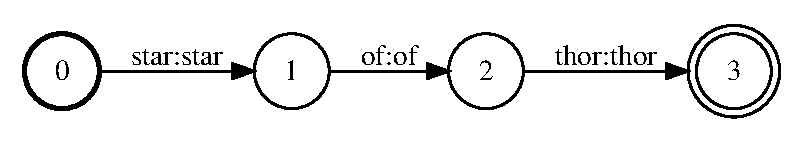
\includegraphics[width=0.95\columnwidth]{figures/fsa}
	\caption{\ac{FSA} for the sentence ``star of thor''.}
	\label{fig:fsa_sentence}
\end{figure}

The most probable sequence of tags can be computed as the shortest path in the \ac{FST} given by the composition:
\begin{equation*}
    \lambda_{sentence} \circ \lambda_{word2concept} \circ \lambda_{concept\_lm}.
\end{equation*}
The shortest path is computed by the \texttt{OpenFst} library using the Viterbi algorithm.
This model is implemented in the file \texttt{model/v1.sh}.

\section{Language Model Improvement}
\label{sec:improvements}

The model presented in \cref{sec:implementation} does not exploit the information provided by the words that are tagged as \texttt{O}.
In fact, all information about the original word is dropped by the transducer $\lambda_{word2concept}$.
We can preserve it by including the word itself in the \texttt{O} tag, so that we can train a more accurate language model.
This idea is implemented in the file \texttt{model/v2.sh}.

Before building the lexicon, the training data is modified to replace the \texttt{O} tags with \texttt{O-word}.
The lexicon, $\lambda_{word2concept}$ and $\lambda_{concept\_lm}$ are build using the modified version of the training data.
Finally, a new transducer $\lambda_{concept2iob}$ is added to translate the \texttt{O-word} tags back to \texttt{O}.
This transducer has a single state $0$, a self transition $\texttt{O-word} \rightarrow \texttt{O}$ for each word in the lexicon and a the self transitions $\texttt{B-concept} \rightarrow \texttt{B}$ and $\texttt{I-concept} \rightarrow \texttt{I}$ for each concept.
All transitions have cost $0$.
For each possible input, there is only one possible transition.

\section{Performances}
\label{sec:performances}

\section{Conclusions}
\label{sec:conclusions}

In this assignment, we created a generative model to do concept tagging.
The best model was the 4-gram model with Kneser-Ney smoothing, trained including the words in the \texttt{O} tags to improve the performances of the underlying concepts language model.
The model was able to reach a F1 score of $82.74\%$ on the test set.


% se metto distribuzione diversa da uniforme per OOV???

\end{document}
